\documentclass{article}
\usepackage{algorithm,algorithmic}
\usepackage{amsmath}
\usepackage{amsthm}
\usepackage{amssymb}
\usepackage{enumerate}
\usepackage[margin=1.00in]{geometry}
\usepackage{graphicx}
\usepackage{hyperref}
\usepackage{tikz}

% new theorems
\newtheorem{theorem}{Theorem}[section]
\newtheorem{proposition}[theorem]{Proposition}
\newtheorem{corollary}[theorem]{Corollary}
\newtheorem{lemma}[theorem]{Lemma}
\newtheorem{example}[theorem]{Example}

\theoremstyle{definition}
\newtheorem{remark}[theorem]{Remark}

% new commands and math operators
\newcommand*\conj[1]{\overline{#1}}
\newcommand{\iu}{{i\mkern1mu}}
\newcommand\abs[1]{\left|#1\right|}
\newcommand\norm[1]{\left\Vert#1\right\Vert}
\newcommand\re[1]{\operatorname{Re}\left(#1\right)}
\newcommand\tr[1]{\operatorname{tr}\left(#1\right)}

\title{A Note to Panos:\\
\emph{\large{Q Numerical Range of the Graph Laplacian}}}
\author{Thomas R. Cameron}
\date{\today}

\begin{document}
\maketitle
\abstract{
This note introduces the Q numerical range of the graph Laplacian and its use for characterizing certain digraphs. 
}

%%%%%%%%%%%%%%%%%%%%%%%%%%%%%%%%%%%%%%%%%%%%%%%%%%%%%%
%                                    				Introduction
%%%%%%%%%%%%%%%%%%%%%%%%%%%%%%%%%%%%%%%%%%%%%%%%%%%%%%
\section{Introduction}	
Let $\Gamma$ be a directed graph (digraph) with non-negative weights and let $L$ be the graph Laplacian of $\Gamma$. 
Furthermore, let $e$ denote the all ones vector. 
Then, the algebraic connectivity of $\Gamma$ is defined as follows~\cite{Wu2005-1}:
\[
\alpha(\Gamma)=\min_{x\in S}x^{T}Lx,
\]
where
\[
S=\left\{x\in\mathbb{R}^{n}\colon x\perp e,\norm{x}=1\right\}.
\]
Another related and useful quantity is the following:
\[
\beta(\Gamma)=\max_{x\in S}x^{T}Lx.
\]
It is important to note that both $\alpha(\Gamma)$ and $\beta(\Gamma)$ are invariant under re-ordering of vertices of $\Gamma$ since the space $S$ is invariant under permutation.

Let $Q$ be an orthonormal matrix whose columns span $S$.
Then, we have
\[
\alpha(\Gamma)=\min_{\norm{Qx}=1}x^{T}Q^{T}LQx
\]
and
\[
\beta(\Gamma)=\max_{\norm{Qx}=1}x^{T}Q^{T}LQx.
\]
Furthermore, let $W(A)$ denote the numerical range (field of values) of a complex matrix $A$, as defined in~\cite{Horn1991}.
Then, the Hermitian part of $A$, denoted $H(A)=\frac{1}{2}(A+A^{*})$, satisfies the following:
\[
W(H(A))=\re{W(A)}.
\]
Moreover, the end points of $\re{W(A)}$ are well-known to be the minimum and maximum eigenvalues of $H(A)$. 
Therefore, we have
\begin{equation}\label{eq:alpha}
\alpha(\Gamma)=\lambda_{\text{min}}\left(\frac{1}{2}Q^{T}(L+L^{T})Q\right)
\end{equation}
and
\begin{equation}\label{eq:beta}
\beta(\Gamma)=\lambda_{\text{max}}\left(\frac{1}{2}Q^{T}(L+L^{T})Q\right).
\end{equation}

%%%%%%%%%%%%%%%%%%%%%%%%%%%%%%%%%%%%%%%%%%%%%%%%%%%%%%
%                                    				The Q Numerical Range of the Graph Laplacian
%%%%%%%%%%%%%%%%%%%%%%%%%%%%%%%%%%%%%%%%%%%%%%%%%%%%%%
\section{The Q Numerical Range of the Graph Laplacian}
Motivated by~\eqref{eq:alpha} and~\eqref{eq:beta}, we are interested in studying the numerical range of the matrix $Q^{T}LQ$, where $L$ is the graph Laplacian of a digraph $\Gamma$ and $Q$ is an orthonormal matrix whose columns span $S$.
We reference the set $W(Q^{T}LQ)$ as the Q numerical range of the graph Laplacian $L$.
The Q numerical range can be used to characterize digraphs and give information about the values of $\alpha(\Gamma)$ and $\beta(\Gamma)$.
For instance, it is easy to show that $W(Q^{T}LQ)=\{0\}$ if and only if $\Gamma$ is the empty graph, and $W(Q^{T}LQ)=\{n\}$ if and only if $\Gamma$ is the complete graph on $n$ vertices.
Therefore, if $\Gamma$ is the empty graph, then $\alpha(\Gamma)=\beta(\Gamma)=0$, and if $\Gamma$ is the complete graph, then $\alpha(\Gamma)=\beta(\Gamma)=n$. 

%%%%%%%%%%%%%%%%%%%%%%%%%%%
%				Directed Cycle				
%%%%%%%%%%%%%%%%%%%%%%%%%%%
\subsection{Directed Cycle}
In this section, we use the Q numerical range to characterize directed cycles and derive $\alpha(\Gamma)$ and $\beta(\Gamma)$ where $\Gamma$ is a directed cycle on $n$ vertices.

%%%%%%%%%%%%%%%%%%%%%%
%			Theorem 2.1			%
%%%%%%%%%%%%%%%%%%%%%%
\begin{theorem}
Let $\Gamma$ be a digraph with binary weights and let $L$ be the graph Laplacian of $\Gamma$.
Then, $\Gamma$ is a directed cycle on $n$ vertices if and only if
\begin{equation}\label{eq:cycle-eig}
\sigma(L)=\left\{1-e^{\iu 2\pi j/n}\colon~j=0,1,\ldots,n-1\right\}.
\end{equation}
\end{theorem}
\begin{proof}
Suppose that $\Gamma$ is a directed cycle on $n$ vertices. 
Then, the graph Laplacian $L=I-A$ is a circulant matrix with first column vector equal to
\[
[1,0,\cdots,0,-1]^{T}.
\]
As a circulant matrix with first column vector defined above, the eigenvalues of $L$ are known to satisfy~\eqref{eq:cycle-eig}. 

Conversely, suppose that the eigenvalues of the graph Laplacian $L$ satisfy~\eqref{eq:cycle-eig}.
Suppose that $0$ is the out-degree of some vertex of $\Gamma$.
Then, $L$ can be written in the form
\[
L=\begin{bmatrix} L_{1} & L_{12} & \cdots & L_{1r} \\ & L_{2} & \cdots & L_{2r} \\ & & \ddots & \vdots \\ & & & 0 \end{bmatrix},
\]
where $L_{1}\oplus L_{2}\oplus\cdots\oplus L_{r-1}$ is a non-singular matrix with eigenvalues 
\[
\left\{1-e^{\iu 2\pi j/n}\colon~j=1,\ldots,n-1\right\}.
\]
For each $k=1,\ldots,r-1$, by~\cite[Lemma 6.4.1]{Berman1994} and~\cite[Theorem 6.2.3 (M35)]{Berman1994}, $L_{k}$ is an irreducible non-singular M-matrix. 
Hence, by~\cite[Theorem 6.2.3 (N38)]{Berman1994}, $L_{k}^{-1}$ exists, is non-negative, and is irreducible.
Now, let $L_{k}$ denote the block with eigenvalue $1-e^{\iu 2\pi/n}$.
Then, by the Perron-Frobenius theorem~\cite[Theorem 2.1.4]{Berman1994}, it follows that $\rho(L_{k}^{-1})$ is a simple eigenvalue.
Since, $1-e^{\iu 2\pi/n}$ is the smallest eigenvalue of $L_{k}$ in magnitude, it follows that $\rho(L_{k}^{-1})=\abs{1/(1-e^{\iu 2\pi/n})}$ is an eigenvalue of $L_{k}^{-1}$. 
However, this is a contradiction and it follows that $0$ is not the out-degree of any vertex of $\Gamma$.

Since $\tr{L}=n$ and the weights of $\Gamma$ are binary, it follows that $d^{+}(i)=1$ for all $i=1,\ldots,n$.
Therefore, $L=I-A$, where the adjacency matrix $A$ has eigenvalues
\[
\left\{e^{\iu 2\pi j/n}\colon~j=0,1,\ldots,n-1\right\}.
\]
Note that $\tr{A^{k}}$ is equal to the number of closed directed walks of length $k$.
Furthermore, $\tr{A^{k}}=0$ if $k<n$ and $A^{n}=I$.
It follows that $\tr{A^{n}}=n$, so there are $n$ directed walks of length $n$.
In fact, there is a walk starting and ending at each vertex.
Since each walk must be in the same direction, it follows that $\Gamma$ is a cycle on $n$ vertices. 
\end{proof}

%%%%%%%%%%%%%%%%%%%%%%
%			Lemma 2.2			%
%%%%%%%%%%%%%%%%%%%%%%
\begin{lemma}\label{lem:normal}
Let $L$ be the graph Laplacian of any digraph.
Then, $L$ is normal if and only if $Q^{T}LQ$ is normal.
\end{lemma}
\begin{proof}
Suppose $L$ is a normal matrix.
Then, $L$ has an orthonormal eigenvector basis for $\mathbb{C}^{n}$, which we denote by $\{v_{1},\ldots,v_{n}\}$, where $v_{n}=e/\sqrt{n}$.
Since the columns of $Q$ are orthogonal to $e$, it follows that for each $j=1,\ldots,n-1$ there is a unique $x_{j}\in\mathbb{C}^{n-1}$ such that $Qx_{j}=v_{j}$.
Therefore, $\{x_{1},\ldots,x_{n-1}\}$ forms an orthonormal basis for $\mathbb{C}^{n-1}$, where each $x_{j}$ is an eigenvector of $Q^{T}LQ$.
Hence, $Q^{T}LQ$ is normal. 

Now, suppose that $Q^{T}LQ$ is normal.
Then, $Q^{T}LQ$ has an orthonormal eigenvector basis for $\mathbb{C}^{n-1}$, which we denote by $\{x_{1},\ldots,x_{n-1}\}$.
Define $v_{j}=Qx_{j}$ for $j=1,\ldots,n-1$, which is a set of $(n-1)$ orthonormal vectors in $\mathbb{C}^{n}$.
Furthermore, each $v_{j}$ is orthogonal to $e$.
Let $v_{n}=e/\sqrt{n}$.
Then, $\{v_{1},\ldots,v_{n}\}$ forms an orthonormal basis for $\mathbb{C}^{n}$, where each $v_{j}$ is an eigenvector of $L$.
Hence, $L$ is normal. 
\end{proof}

%%%%%%%%%%%%%%%%%%%%%%
%			Theorem 2.3			%
%%%%%%%%%%%%%%%%%%%%%%
\begin{theorem}\label{thm:cycle-qnr}
Let $\Gamma$ be a directed cycle with binary weights and let $L$ be the graph Laplacian of $\Gamma$.
Then, $\Gamma$ is a directed cycle if and only if $W(Q^{T}LQ)$ is polygon with vertices
\[
\left\{1-e^{\iu 2\pi j/n}\colon~j=1,\ldots,n-1\right\}.
\]
\end{theorem}
\begin{proof}
Suppose that $\Gamma$ is a directed cycle.
Then, the graph Laplacian $L=I-A$ is a circulant matrix with first column vector equal to
\[
[1,0,\ldots,0,-1]^{T}.
\]
As a circulant matrix, $L$ has eigenvectors that form an orthonormal basis for $\mathbb{C}^{n}$ and is therefore normal.
Furthermore, since the first column vector of $L$ is equal to the vector above, it follows that the eigenvalues of $L$ satisfy~\eqref{eq:cycle-eig}. 
Therefore, by Lemma~\ref{lem:normal}, $Q^{T}LQ$ is a normal matrix with eigenvalues that satisfy
\[
\sigma(Q^{T}LQ)=\{1-e^{\iu 2\pi j/n}\colon~j=1,\ldots,n-1\}.
\]
Hence, $W(Q^{T}LQ)$ is equal to the convex hull of $\sigma(Q^{T}LQ)$. 

Conversely, suppose that $W(Q^{T}LQ)$ is a polygon with vertices
\[
\{1-e^{\iu 2\pi j/n}\colon~j=1,\ldots,n-1\}.
\]
Then, these $(n-1)$ vertices are the eigenvalues of $Q^{T}LQ$.
Therefore, the eigenvalues of $L$ satisfy~\eqref{eq:cycle-eig}, and it follows that $\Gamma$ is a cycle on $n$ vertices. 
\end{proof}

Finally, the corollary below follows from Theorem~\ref{thm:cycle-qnr} and~\eqref{eq:alpha} and~\eqref{eq:beta}.
%%%%%%%%%%%%%%%%%%%%%%
%			Corollary 2.4			%
%%%%%%%%%%%%%%%%%%%%%%
\begin{corollary}\label{cor:cycle-alpha-beta}
If $\Gamma$ is a directed cycle on $n$ vertices, then
\[
\alpha(\Gamma) = 1-\re{e^{\iu 2\pi/n}}
\]
and
\[
\beta(\Gamma) = \begin{cases} 
				2 & \text{if $n$ is even}, \\
				1 - \re{e^{\iu \pi (n-1)/n}} & \text{if $n$ is odd}.
				\end{cases}
\]
\end{corollary}

%%%%%%%%%%%%%%%%%%%%%%%%%%%
%			The Imploding Star		
%%%%%%%%%%%%%%%%%%%%%%%%%%%
\subsection{The Imploding Star}
The imploding star on $4$ vertices is shown below.
%%%%%%%%%%%%%%%%%%%%%%
%			Figure 1				%
%%%%%%%%%%%%%%%%%%%%%%
\begin{figure}[ht]
\centering
\resizebox{0.20\textwidth}{!}{% complete dominance
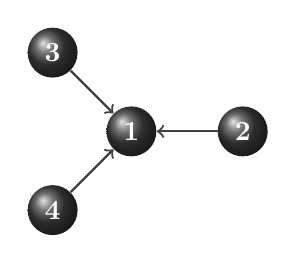
\begin{tikzpicture}
	\node[circle, shading=ball, ball color=black!75, color=white] (1) at (0,0) {\textbf{1}};
	\node[circle, shading=ball, ball color=black!75, color=white] (2) at (1.414,0) {\textbf{2}};
	\node[circle, shading=ball, ball color=black!75, color=white] (3) at (-1,1) {\textbf{3}};
	\node[circle, shading=ball, ball color=black!75, color=white] (4) at (-1,-1) {\textbf{4}};
	
	% vertex 1
	% vertex 2
	\draw[black!75,->,thick](2) to [out=180,in=0,looseness=0](1);
	% vertex 3
	\draw[black!75,->,thick](3) to [out=315,in=135,looseness=0](1);
	% vertex 4
	\draw[black!75,->,thick](4) to [out=45,in=225,looseness=0](1);
\end{tikzpicture}%
}
\caption{Imploding star on $4$ vertices.}
\label{fig:imp-star}
\end{figure}
In this section, we use the Q numerical range to characterize the imploding star and derive values for $\alpha(\Gamma)$ and $\beta(\Gamma)$ where $\Gamma$ is an imploding star on $n\geq 3$ vertices.
It is important to note that the imploding star is not characterized by its Laplacian spectrum. 

%%%%%%%%%%%%%%%%%%%%%%
%			Theorem 2.5			%
%%%%%%%%%%%%%%%%%%%%%%
\begin{theorem}\label{thm:imp-star}
Let $\Gamma$ be a directed graph with binary weights and let $L$ be the graph Laplacian of $\Gamma$.
Then, $\Gamma$ is an imploding star if and only if $W(Q^{T}LQ)=\{1\}$. 
\end{theorem}
\begin{proof}
Let $\Gamma$ be an imploding star.
Then, the graph Laplacian of $\Gamma$ can be written in the form
\[
L=\begin{bmatrix} 1 & 0 & \cdots & 0 & -1 \\ & 1 & \cdots & 0 & -1 \\ & & \ddots & \vdots & \vdots \\ & & & 1 & -1 \\ & & & & 0 \end{bmatrix} = I - ee_{n},
\]
where $I$ is the identity matrix, $e$ is the vector of all ones, and $e_{n}$ is the $n$th standard basis vector of $\mathbb{R}^{n}$.

Denote the columns of $Q$ by $\{q_{1},\ldots,q_{n-1}\}$ and recall that these vectors form an orthonormal basis for $S$.
Note that, for $j=1,\ldots,n-1$, we have
\begin{align*}
Lq_{j} &= q_{j} - ee_{n}q_{j} \\
&= q_{j} - q_{j}(n)e. 
\end{align*}
Since the vectors in $S$ are all orthogonal to $e$, it follows that
\[
q_{i}^{T}Lq_{j}=\begin{cases}
				1 & \text{if $i=j$}, \\
				0 & \text{if $i\neq j$}.
			\end{cases}
\]
Therefore, $Q^{T}LQ$ and it follows that $W(Q^{T}LQ)=\{1\}$. 

Conversely, suppose that $W(Q^{T}LQ)=\{1\}$. 
Then, $Q^{T}LQ=I$, and it follows that the eigenvalues of $L$ satisfy
\[
\sigma(L)=\{0,1\},
\]
where $1$ is repeated $(n-1)$ times.

Now, suppose that $\Gamma$ is not acyclic.
Then, there exists a strongly connected component $\Gamma_{k}$ made up of $m$ vertices, where $m\geq 2$. 
If $L_{k}$ has a zero eigenvalue, then $\tr{L}>n-1$ since $\gamma$ has binary weights and no diagonal entry of $L$ is equal to zero.
If $L_{k}$ has no zero eigenvalue, then one of the diagonal entries of $L_{k}$ must be greater than one, and it follows that $\tr{L}>n-1$. 
Hence, in either case, we have a contradiction.
Therefore, $\Gamma$ is acyclic. 

It follows that $L$ can be written in the form
\[
L=\begin{bmatrix} 1 & l_{12} & \cdots & l_{1(n-1)} & l_{1n} \\ & 1 & \cdots & l_{2(n-1)} & l_{2n} \\ & & \ddots & & \\ & & & 1 & -1 \\ & & & & 0\end{bmatrix}
\]
Without loss of generality, assume that
\[
Q=\begin{bmatrix} \frac{1}{\sqrt{2}} & \frac{1}{\sqrt{6}} & \cdots & \frac{1}{\sqrt{(n-1)^{2}+(n-1)}} \\ \frac{-1}{\sqrt{2}} & \frac{1}{\sqrt{6}} & \cdots & \frac{1}{\sqrt{(n-1)^{2}+(n-1)}} \\ & \frac{-2}{\sqrt{6}} & \cdots & \frac{1}{\sqrt{(n-1)^{2}+(n-1)}} \\ & & & \vdots \\ & & & \frac{-(n-1)}{\sqrt{(n-1)^{2}+(n-1)}} \end{bmatrix}.
\]
Then, writing out the entry-wise equations of $Q^{T}LQ=I$, it is clear that
\[
l_{ij} = 	\begin{cases}
		0 & \text{if $1\leq i\leq n-2$ and $i<j<n$}, \\
		-1 & \text{if $1\leq i\leq n-2$ and $j=n$}.
		\end{cases}
\]
Therefore, $\Gamma$ is an imploding star. 
\end{proof}

We have the following immediate corollary of Theorem~\ref{thm:imp-star}.
%%%%%%%%%%%%%%%%%%%%%%
%			Theorem 2.6			%
%%%%%%%%%%%%%%%%%%%%%%
\begin{corollary}\label{thm:imp-star-alpha-beta}
Let $\Gamma$ be an imploding star.
Then, $\alpha(\Gamma)=\beta(\Gamma)=1$. 
\end{corollary}

Finally, it is worth noting that the imploding star is not characterized by its Laplacian spectrum.
For instance, note that the following graph is not isomorphic to the imploding star in Figure~\ref{fig:imp-star} but has the same Laplacian spectrum of $\{1,1,1,0\}$.
%%%%%%%%%%%%%%%%%%%%%%
%			Figure 2				%
%%%%%%%%%%%%%%%%%%%%%%
\begin{figure}[ht]
\centering
\resizebox{0.20\textwidth}{!}{% complete dominance
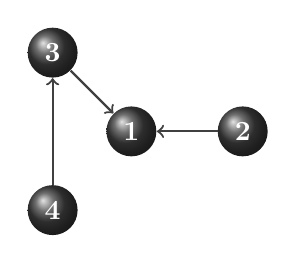
\begin{tikzpicture}
	\node[circle, shading=ball, ball color=black!75, color=white] (1) at (0,0) {\textbf{1}};
	\node[circle, shading=ball, ball color=black!75, color=white] (2) at (1.414,0) {\textbf{2}};
	\node[circle, shading=ball, ball color=black!75, color=white] (3) at (-1,1) {\textbf{3}};
	\node[circle, shading=ball, ball color=black!75, color=white] (4) at (-1,-1) {\textbf{4}};
	
	% vertex 1
	% vertex 2
	\draw[black!75,->,thick](2) to [out=180,in=0,looseness=0](1);
	% vertex 3
	\draw[black!75,->,thick](3) to [out=315,in=135,looseness=0](1);
	% vertex 4
	\draw[black!75,->,thick](4) to [out=90,in=270,looseness=0](3);
\end{tikzpicture}%
}
\caption{Digraph not isomorphic to imploding star with the same Laplacian spectrum.}
\label{fig:niso-imp-star}
\end{figure}

%%%%%%%%%%%%%%%%%%%%%%%%%%%
%			The Exploding Star		
%%%%%%%%%%%%%%%%%%%%%%%%%%%
\subsection{The Exploding Star}

%%%%%%%%%%%%%%%%%%%%%%%%%%%%%%%%%%%%%%%%%%%%%%%%%%%%%%
%                                 	   			Bibliography
%%%%%%%%%%%%%%%%%%%%%%%%%%%%%%%%%%%%%%%%%%%%%%%%%%%%%%
\label{Bibliography}
\bibliographystyle{siam}
\bibliography{Bibliography}

\end{document}